% !TeX root = ../tfg.tex
% !TeX encoding = utf8

\chapter{Probabilidad}\label{ch:capitulo-teoria-de-la-probabilidad}

En este capítulo se presentarán algunas definiciones y resultados de la teoría de la probabilidad y la estadística, con el propósito de introducir conceptos clave que faciliten la comprensión del \textit{Deep Double Descent} y que utilizaremos a lo largo del desarrollo de gran parte del trabajo. Las fuentes principales utilizadas a lo largo de este capítulo son extractos de~\cite{Dembo2014, Knill2009}.

\section{Espacios de probabilidad y $\sigma$-álgebras}

Para establecer la base teórica, consideraremos un conjunto arbitrario $\Omega$, al que nos referiremos como \textbf{espacio muestral} y que representa el conjunto de todos los posibles resultados al realizar un experimento. Asimismo, llamaremos \textbf{suceso} a cualquier subconjunto de $\Omega$.

\begin{definicion}[$\sigma$-álgebra]\label{def:sigma-algebra}
    Un conjunto $\mathcal{A}$ de subconjuntos de $\Omega$ ($\mathcal{A} \subseteq \mathcal{P}(\Omega)$) se dirá que es una \emph{$\sigma$-álgebra} si verifica las siguientes propiedades:

    \begin{enumerate}
        \item $\Omega \in \mathcal{A}$.
        \item Si $\mathrm{A} \in \mathcal{A}$, entonces $\mathrm{A}^c = \Omega \setminus \mathcal{A} \in \mathcal{A}$ ($\mathrm{A}$ es cerrado bajo complementarios).
        \item Si $\mathrm{A}_{n} \in \mathcal{A}$, entonces $\bigcup_{n \in \mathbb{N}} \mathrm{A}_{n} \in \mathcal{A}$ (A es cerrado bajo uniones finitas).
    \end{enumerate}
\end{definicion}

Es fácil comprobar que $\mathcal{A}$ es cerrado bajo intersecciones finitas y que, además, la intersección de $\sigma$-álgebras es una $\sigma$-álgebra.

\begin{definicion}[$\sigma$-álgebra de Borel]\label{def:sigma-algebra-borel}
    Para cada conjunto $\mathcal{C}$ de subconjuntos de $\Omega$, se define $\sigma(\mathcal{C})$ como la menor $\sigma$-álgebra $\mathcal{A}$ que contiene a $\mathcal{C}$. La $\sigma$-álgebra $\mathcal{A}$ es la intersección de todas las $\sigma$-álgebras que contienen a $\mathcal{C}$ y, por tanto, es una $\sigma$-álgebra.

    Si ($\mathrm{E}, \mathcal{O}$) es un espacio topológico, donde $\mathrm{O}$ es el conjunto formado por los conjuntos abiertos en E, entonces $\sigma(\mathcal{O})$ es llamada la \textbf{$\sigma$-álgebra de Borel} del espacio topológico.
\end{definicion}

Llamaremos \textbf{espacio de medida} al conjunto ($\Omega, \mathcal{A}$) donde $\mathcal{A}$ es una $\sigma$-álgebra en $\Omega$.

\begin{definicion}[Medida de probabilidad]\label{def:medida-de-probabilidad}
    Dado un espacio de medida ($\Omega, \mathcal{A}$), una función $\mathrm{P}: \mathcal{A} \to \mathbb{R}$ se llamará \emph{medida de probabilidad} si cumple las siguientes tres propiedades (conocidas como \textbf{axiomas de Kolmogorov}~\cite{Kolmogorov1956}):

    \begin{enumerate}
        \item $\mathrm{P}[\mathrm{A}] \ge 0$ para todo $\mathrm{A} \in \mathcal{A}$.
        \item $\mathrm{P}[\Omega]=1$.
        \item $\mathrm{P}$ es $\sigma$-aditiva, es decir, si $\mathrm{A}_n \in \mathcal{A}$ con $n \in \mathbb{N}$ son conjuntos disjuntos dos a dos, entonces 
        \[ \mathrm{P}\left[\bigcup_{n \in \mathbb{N}} \mathrm{A}_{n}\right] = \sum\limits_{n \in \mathbb{N}} \mathrm{P}[\mathrm{A}_n]. \]
    \end{enumerate}
\end{definicion}

La primera condición nos asegura la no negatividad de la probabilidad, es decir, la probabilidad nunca será inferior a $0$. A su vez, la segunda condición nos establece que la probabilidad del espacio muestral completo ($\Omega$) debe ser igual a $1$, es decir, refleja que uno de los eventos posibles siempre ocurrirá, conocido como \textbf{suceso seguro}.

\begin{observacion}
Como consecuencia de las propiedades $2$ y $3$ de la definición anterior, se sigue de manera inmediata que $\mathrm{P}(\emptyset) = 0$. Además, al conjunto $\emptyset$ se le suele denominar como \emph{evento imposible}.
\end{observacion}

\begin{corolario}\label{cor:propiedades-adicionales}
    Algunas propiedades básicas de la medida de probabilidad ($\mathrm{P}$) que se siguen de la propia definición son las siguientes:

    \begin{enumerate}
        \item Si $\mathrm{A}, \mathrm{B} \in \mathcal{A}$ y $\mathrm{A} \subset B$, entonces $\mathrm{P}[\mathrm{A}] \le \mathrm{P}[\mathrm{B}]$.
        \item $\mathrm{P}[\mathrm{A^c}] = 1-\mathrm{P}[\mathrm{A}]$, para todo $\mathrm{A} \in \mathcal{A}$.
        \item $0 \le \mathrm{P}[\mathrm{A}] \le 1$, para todo $\mathrm{A} \in \mathcal{A}$.
    \end{enumerate}
\end{corolario}

\begin{observacion}
Existen distintas formas de construir los axiomas para un espacio de probabilidad. Por ejemplo, se podrían sustituir las primeras dos propiedades de la definición de medida de probabilidad por las últimas dos propiedades enunciadas en el corolario anterior.
\end{observacion}

\begin{definicion}[Espacio de probabilidad]\label{def:espacio-de-probabilidad}
    Dado un espacio de medida ($\Omega, \mathcal{A}$), llamaremos \emph{espacio de probabilidad} a la tripleta ($\Omega, \mathcal{A}, \mathrm{P}$), donde $\mathrm{P}$ es una medida de probabilidad.
\end{definicion}

\section{Variables aleatorias y esperanza}

Las variables aleatorias son funciones numéricas que asignan un valor numérico a cada posible resultado de un experimento aleatorio $w \in \Omega$. De manera intuitiva, una variable aleatoria puede verse como una cantidad numérica cuyo valor no es fijo y que puede tomar distintos valores, por lo que es necesario definir una distribución de probabilidad que asocie probabilidades a los distintos valores que pueda tomar la variable aleatoria. 

\begin{definicion}[Función medible]\label{def:funcion-medible}
    Una función $X: (\Omega_1, \mathcal{A}) \to (\Omega_2, \mathcal{B})$ se dice \emph{medible} si

    \[ X^{-1}(\mathrm{B}) \in \mathcal{A}, \quad \forall \mathrm{B}  \in \mathcal{B}, \]

    donde el conjunto $ X^{-1}(\mathrm{B})$ se encuentra formado por todos los puntos $x \in \Omega$ para los cuales $X(x) \in \mathrm{B}$.
\end{definicion}

\begin{definicion}[Variable aleatoria]\label{def:variable-aleatoria}
    Dado un espacio de probabilidad ($\Omega_1, \mathcal{A}, \mathrm{P}$) y un espacio medible ($\Omega_2, \mathcal{B}$), decimos que $X: (\Omega_1, \mathcal{A}, \mathrm{P}) \to (\Omega_2, \mathcal{B})$ es una \emph{variable aleatoria} si $X$ es una función medible.
\end{definicion}

Además, si el espacio medible de llegada es $n$-dimensional, entonces la variable aleatoria $X$ es llamada \textbf{vector aleatorio} y lo denotaremos por $X = (X_1, X_2, \ldots, X_n)$, donde cada componente $X_i$, con $i \in \{1, 2, \ldots, n\}$, es una variable aleatoria.

\begin{observacion}
    En la mayoría de usos prácticos se tiene que el espacio medible de llegada más común es ($\mathbb{R}, \mathcal{B}(\mathbb{R})$), donde $\mathcal{B}(\mathbb{R})$ denota la $\sigma$-álgebra de Borel en $\mathbb{R}$.
\end{observacion}

\begin{definicion}
    Diremos que una variable aleatoria es \emph{discreta} si esta toma un número finito o numerable de valores en el espacio de llegada. Por otra parte, si la variable aleatoria toma un número infinito o no numerable de valores, diremos que es una variable aleatoria \emph{continua}.
\end{definicion}

\begin{ejemplo}
    Como ejemplo sencillo podemos considerar los posibles resultados obtenidos al lanzar un dado de seis caras, es decir, $w \in \{1,2,3,4,5,6\}$, y podemos definir la variable aleatoria discreta que asigna a cada resultado el valor de la cara superior obtenida al realizar el lanzamiento. En este caso, la variable aleatoria se define como:

    \[ X(w) = w, \quad \text{para} \; w \in \{1,2,3,4,5,6\}. \]
\end{ejemplo}

\begin{definicion}[Función de distribución]\label{def:funcion-de-distribucion}
    La \emph{función de distribución (acumulada)} de una variable aleatoria $X$ es la función $F_X: \mathbb{R} \to [0,1]$ definida por:

    \[ F_X(\alpha) = P[\{ w:X(w) \le \alpha\}], \quad \forall \alpha \in \mathbb{R}. \]
\end{definicion}

\begin{proposicion}
    La función de distribución $F$ de una variable aleatoria $X$ cumple las siguientes propiedades:

    \begin{enumerate}
        \item $F$ es monótona no decreciente.
        \item $\lim_{x \to \infty} F(x) = 1$ y $\lim_{x \to -\infty} F(x) = 0$.
        \item $F$ es continua por la derecha, es decir, $\lim_{y \to x^+} F(y) = F(x)$.
    \end{enumerate}
\end{proposicion}

\begin{definicion}[Función de probabilidad]\label{def:funcion-de-probabilidad}
    Sea $X$ una variable aleatoria discreta, llamaremos \emph{función (masa) de probabilidad} a la función que asigna la probabilidad de que la variable aleatoria tome un valor en particular, es decir:

    \[ p_X(x) = P[X = x], \quad \text{con} \; x \in \{x_1, \ldots, x_n\}. \]
\end{definicion}

Las probabilidades asociadas con todos los posibles resultados del experimento deben ser no negativas y sumar uno, es decir $ \sum_x p_X(x) = 1 $ y, además, $p_X(x) \ge 0$.

Notemos que el concepto de función de probabilidad solo tiene sentido al hablar de variables aleatorias discretas. Para variables aleatorias continuas, el concepto análogo es el de función de densidad, donde deberemos integrar para obtener la probabilidad, pues la probabilidad asociada a un único punto en un intervalo es cero.

\begin{definicion}[Función de densidad]\label{def:funcion-de-densidad}
    Se dice que una función $f_X$, integrable de Lebesgue y no negativa en casi todas partes, es la \emph{función de densidad} de una variable aleatoria continua $X$ si su función de distribución puede ser expresada como

    \[ F_X(\alpha) =  \int_{-\infty}^{\alpha} f_X(x) \, dx, \quad \forall \alpha \in \mathbb{R}. \]
\end{definicion}

Notemos que la función de densidad, de manera análoga a la función de probabilidad, cumple $ f_X(x) \ge 0$ y $ \int_{-\infty}^{\infty} f_X(x) \, dx = 1$.

\begin{definicion}[\textbf{Esperanza de una variable aleatoria}]\label{def:esperanza-variable-aleatoria}
Sea $X$ una variable aleatoria en el espacio de probabilidad ($\Omega, \mathcal{A}, \mathrm{P}$). Definimos el \textbf{valor esperado o esperanza} de $X$, denotada por $E[X]$, como la integral de Lebesgue siguiente:

\[ \mathbb{E}[X] = \int_{\Omega} X(w) \, dP[w]. \]

Para vectores aleatorios, su esperanza viene definida componente a componente:

\[ \mathbb{E}[(X_1, \ldots, X_n)] = (\mathbb{E}[X_1], \ldots, \mathbb{E}[X_n]). \]
\end{definicion}

\begin{observacion}
    Si $X$ es una variable aleatoria discreta con función de probabilidad $\mathrm{P}[X = x_i]$, con $i \in \{1,2,\ldots,n\}$, su esperanza viene definida por:

    \[ \mathbb{E}[X] = \sum_{i=1}^{n} x_i \: \mathrm{P}[X = x_i], \]

    donde $x_i$ denota cada posible resultado del experimento.
\end{observacion}

\begin{observacion}
    Si $X$ es una variable aleatoria continua con función de densidad $f_X(x)$, su esperanza se define como:

    \[ \mathbb{E}[X] =  \int_{\mathbb{R}} x f_X(x) \, dx. \]
\end{observacion}

\subsection{Probabilidad condicional}

En esta sección introduciremos la noción clásica de \emph{probabilidad condicional} de sucesos, ligada al supuesto de conocer la probabilidad de un cierto suceso bajo la condición de que ocurra otro suceso. De igual manera, se introducirán resultados necesarios para el desarrollo del trabajo, tales como el teorema de Bayes.

\begin{definicion}[Probabilidad condicional]\label{def:probabilidad-condicional}
    Dados dos sucesos $A, B \in \mathcal{A}$ con $P[B] > 0$, definimos la \emph{probabilidad condicional} de $A$ con respecto a $B$ de la siguiente forma:

    \[ P[A|B] = \frac{P[A \cap B]}{P[B]}. \]
\end{definicion}

\begin{definicion}\label{def:particion-finita}
    Un conjunto finito $\{A_1, \ldots, A_n \} \subset \mathcal{A}$ se denominará \emph{partición finita} de $\Omega$ si cumple:

    \begin{enumerate}
        \item $\bigcup\limits_{i=1}^n A_i = \Omega$.
        \item $A_i \cap A_j = \emptyset$, para todo $i \neq j$.
    \end{enumerate}
\end{definicion}

Una partición finita cubre todo el espacio con un número finito de conjuntos (sucesos) disjuntos dos a dos.

\begin{teorema}[Probabilidad total]\label{teo:probabilidad-total}
    Sean $\{A_1, \ldots, A_n \}$ una partición finita de $\mathcal{A}$ y $B \in \mathcal{A}$ un suceso cualquiera del que se conocen las probabilidades condicionales $P[B|A_i] \; \forall i \in \{1, \ldots, n \}$. Entonces, la probabilidad del suceso $B$ viene dada por la siguiente expresión:

    \[ P[B] = \sum_{i=1}^{n} P[B|A_i]P[A_i]. \]
\end{teorema}

\begin{proof}
    Partimos de una partición finita $\{A_1, \ldots, A_n \}$ de $\mathcal{A}$ y de un suceso $B \in \mathcal{A}$. Usando la primera propiedad de la Definición~\ref{def:particion-finita}, podemos expresar el suceso B de la siguiente forma:

    \[ B = (B \cap A_1) \cup (B \cap A_2) \cup \cdots \cup (B \cap A_n). \]

    Utilizando la segunda propiedad de la Definición~\ref{def:particion-finita}, sabemos que $A_i \cap A_j = \emptyset, i \neq j$. Por tanto, obtenemos que los conjuntos $(B \cap A_i), \; i \in \{1, \ldots, n\}$ son, también, disjuntos dos a dos.

    Por consiguiente, podemos expresar la probabilidad del suceso $B$ como sigue:

    \[ P[B] = P[B \cap A_1] + P[B \cap A_2] + \cdots + P[B \cap A_n]. \]

    A continuación, usando la Definición~\ref{def:probabilidad-condicional}, obtenemos que 
    \[ P[A_i \cap B] = P[A_i | B]P[B],\quad \forall i \in \{1, \ldots, n\}. \]
    
    Finalmente, obtenemos la expresión buscada:
    \begin{align*}
        P[B] &= P[B \cap A_1] + P[B \cap A_2] + \cdots + P[B \cap A_n] \\
             &= P[B|A_1]P[A_1] + P[B|A_2]P[A_2] + \cdots + P[B|A_n]P[A_n] \\
             &= \sum_{i=1}^n P[B|A_i]P[A_i].
    \end{align*}
\end{proof}

Llegados a este punto estamos en las condiciones necesarias de introducir un teorema fundamental que nos permite calcular probabilidades condicionales. Este resultado vincula la probabilidad de un suceso $A$ dado otro suceso $B$ ($P[A|B]$) con la probabilidad del suceso $B$ dado el suceso $A$ ($P[B|A]$).

\begin{teorema}[Regla de Bayes]\label{teo:teorema-de-bayes}
    Dada una partición finita $\{A_1, \ldots, A_n \}$ de $\mathcal{A}$ y un suceso $B \in \mathcal{A}$ con $P[B] > 0$, se verifica:

    \[ P[A_i | B] = \frac{P[B | A_i]P[A_i]}{\sum_{i=1}^n P[B|A_i]P[A_i]}. \]
\end{teorema}

\begin{proof}
    En primer lugar, de la Definición~\ref{def:probabilidad-condicional}, sabemos que
     $P[A_i|B] = \frac{P[A_i \cap B]}{P[B]}$. Además, del Teorema~\ref{teo:probabilidad-total}, conocemos que $P[B] = \sum_{i=1}^n P[B|A_i]P[A_i]$.

    Por otra parte, podemos aplicar la Definición~\ref{def:probabilidad-condicional} de la siguiente manera:

    \[ P[B|A_i] = \frac{P[B \cap A_i]}{P[A_i]}. \]

    Ahora, despejando, obtenemos $P[A_i \cap B] = P[B \cap A_i] = P[B|A_i]{P[A_i]}$. Finalmente, combinado ambos resultados alcanzamos la conclusión buscada:

    \[ P[A_i|B] = \frac{P[A_i \cap B]}{P[B]} = \frac{P[B | A_i]P[A_i]}{\sum_{i=1}^n P[B|A_i]P[A_i]}. \]
    
\end{proof}

\subsection{Independencia de variables aleatorias}

En esta sección nos centraremos en explicar el concepto de independencia en el contexto de variables aleatorias. De manera intuitiva, el concepto de independencia, como su nombre indica, va ligado al hecho de que el conocimiento que poseamos de una de las variables no proporciona información adicional sobre el conocimiento de la otra. Para ello, también expandiremos el concepto de función de distribución para el caso de más de una variable aleatoria (vector aleatorio).

\begin{definicion}[Función de distribución conjunta]\label{def:funcion-de-distribucion-conjunta}
    Sean $X_1, \ldots, X_n$ variables aleatorias definidas sobre el mismo espacio de probabilidad $(\Omega, \mathcal{A}, \mathrm{P})$, la \emph{función de distribución conjunta} es la función $F_{X_{1}, \ldots, X_{n}}: \mathbb{R} \to [0,1]$ definida por

    \[ F_{X_{1}, \ldots, X_{n}}(x_1, \ldots, x_n) = P[X_1 \leq x_1, \ldots, X_n \leq x_n], \quad x_1, \ldots, x_n \in \mathbb{R}. \]

    Si interpretamos las $n$ variables aleatorias como un vector aleatorio $X = (X_1, \ldots, X_n)$, podemos simplificar la notación de la siguiente forma:

    \[ F_{X_{1}, \ldots, X_{n}}(x_1, \ldots, x_n) = F_X(x_1, \ldots, x_n). \]
\end{definicion}

De la misma forma, podemos extender las definiciones de \emph{función de probabilidad} y \emph{función de densidad} para el caso en el que dispongamos de más de una variable aleatoria.

En primer lugar, comenzaremos definiendo y demostrando el resultado de la \textbf{regla de la cadena} para probabilidades, que nos será de gran utilidad para trabajar con las siguientes definiciones.

\begin{teorema}[Regla de la cadena]
    Sea ($\Omega, \mathcal{A}, P$) un espacio de probabilidad y $\{A_1, \ldots, A_n \} \in \mathcal{A}$ una serie de sucesos. Entonces, se verifica

    \[ P[A_1 \cap A_2 \cap \ \ldots \ \cap A_n] =  P[A_1]P[A_2 | A_1]\cdots \prod_{i=2}^n P[A_i | A_1 \ \cap \cdots \ \cap A_{i-1}]. \]
\end{teorema}

\begin{proof}
    La demostración se realiza de manera sencilla por recursión, teniendo en cuenta que en el primer caso se hace uso de la Definición~\ref{def:probabilidad-condicional}:

    \[ P[A_1 \cap A_2] = P[A_1]P[A_2| A_1]. \]
\end{proof}

\begin{definicion}[Función de probabilidad conjunta]
    Sean $X_1, \ldots, X_n$ variables aleatorias discretas. La \emph{función (masa) de probabilidad conjunta} de dichas variables viene dada por

    \[ p_{X_1, \ldots, X_n}(x_1, \ldots, x_n) = P[X_1 = x_1, \ldots, X_n = x_n], \quad (x_1, \ldots, x_n) \in \mathbb{R}^n. \]

    Equivalentemente, la función de probabilidad conjunta puede ser expresada de la siguiente forma:

    \begin{align*}
        p_{X_1, \dots, X_n}(x_1, \dots, x_n) &= P(X_1 = x_1) \cdot P(X_2 = x_2 \mid X_1 = x_1) \cdot \\
        &\quad \cdot P(X_3 = x_3 \mid X_1 = x_1, X_2 = x_2) \cdots \\
        &\quad \cdot P(X_n = x_n \mid X_1 = x_1, X_2 = x_2, \dots, X_{n-1} = x_{n-1}),
    \end{align*}

    donde se utiliza la definición de probabilidad condicionada y la regla de la cadena comentada en el teorema anterior.
\end{definicion}

Además, dado que estamos trabajando con probabilidades, se verifica que la suma total debe ser igual a uno, es decir 
\[ \sum_{i}\sum_{j}\ldots\sum_{k}P[X_1=x_{1i}, X_2=x_{2j}, \ldots, X_n=x_{nk}] = 1, \] 
donde los distintos índices ($i, j, \ldots, k$) recorren todos los posibles resultados de cada variable aleatoria.

\begin{definicion}[Función de densidad conjunta]
    Sean $X_1, \ldots, X_n$ variables aleatorias continuas. Se dice que una función $f_{X_{1}, \ldots, X_n}$, integrable de Lebesgue y no negativa en casi todas partes, es la \emph{función de densidad conjunta} de las variables aleatorias continuas $X_1, \ldots, X_n$ si la función de distribución conjunta puede ser expresada como

    \begin{align*}
        F_{X_{1}, \ldots, X_{n}}(x_1, \ldots, x_n) &=  
        \int_{-\infty}^{x_1} \cdots \int_{-\infty}^{x_n} 
        f_{X_{1}, \ldots, X_n}(x_1, \ldots, x_n) \, dx_1 \cdots dx_n, \\
        &\quad \forall(x_1, \ldots, x_n) \in \mathbb{R}^n.
    \end{align*}

    Una manera análoga de expresar la función de densidad conjunta es la siguiente:

    \[ f_{X_{1}, \ldots, X_n} (x_1, \ldots, x_n) = \frac{\partial^{n}F_{X_{1}, \ldots, X_{n}}(x_1, \ldots, x_n)}{\partial x_1 \ldots \partial x_n}. \]
\end{definicion}

De manera análoga a la definición anterior y dado que estamos trabajando con distribuciones de probabilidad, se verifica que 

\[ \int_{-\infty}^{x_1} \cdots \int_{-\infty}^{x_n} f_{X_{1}, \ldots, X_n} (x_1, \ldots, x_n) \, dx_1 \cdots dx_n = 1. \]


Una vez conocemos las funciones conjuntas de una serie de variables aleatorias, es posible determinar la probabilidad de un suceso sin considerar la influencia de otras variables por medio de las funciones marginales.

\begin{definicion}[Función de distribución marginal]
    Sean $X_1, \ldots, X_n$ variables aleatorias. Se define la \emph{función de probabilidad marginal} de la variable aleatoria $X_i$, para $i \in \{1, \ldots, n\}$, de la siguiente manera:

    \[ \forall i = \{1,\ldots,n\},  \qquad F_{X_i}(x_i) = F_{X_{1}, \ldots, X_{n}}(+\infty, \ldots,x_i, \ldots,+\infty), \quad \forall x_i \in \mathbb{R}. \]
\end{definicion}

\begin{definicion}[Función de probabilidad marginal]
    Sean $X_1, \ldots, X_n$ variables aleatorias discretas. Se define la \emph{función (masa) de probabilidad marginal} de la variable aleatoria $X_i$, para $i \in \{1, \ldots, n\}$, de la siguiente forma:

    \[ p_{X_i}(x_i) = \sum_{x_1}\ldots\sum_{x_{i-1}}\sum_{x_{i+1}}\ldots\sum_{x_{n}} p_{X_1, \ldots, X_n}(x_1, \ldots, x_n), \quad (x_1, \ldots, x_n) \in \mathbb{R^n}. \]
\end{definicion}

\begin{definicion}[Función de densidad marginal]
    Sean $X_1, \ldots, X_n$ variables aleatorias continuas. Se define la \emph{función de densidad marginal} de la variable aleatoria $X_i$, para $i \in \{1, \ldots, n\}$, como sigue:

    \[ f_{X_i}(x_i) = \int_{-\infty}^{x_1} \cdots \int_{-\infty}^{x_n} f_{X_{1}, \ldots, X_n} (x_1, \ldots, x_n) \, dx_1 \cdots dx_{i-1} dx_{i+1} \cdots  dx_n, \quad \forall x_i \in \mathbb{R}. \]
\end{definicion}

\begin{definicion}\label{def:variables-aleatorias-idénticamente-distribuidas}
    Sean $X_1, \ldots, X_n$ variables aleatorias definidas sobre el mismo espacio de probabilidad $(\Omega, \mathcal{A}, \mathrm{P})$, con funciones de distribución $F_{X_1}, \ldots, F_{X_n}$ respectivamente. Decimos que las variables aleatorias son \textbf{idénticamente distribuidas (i.d.)} si

    \[ F_{X_1}(x) = F_{X_j}(x), \quad \forall j \in \{1, \ldots, n \} \; y \; \forall x \in \mathbb{R}. \]
\end{definicion}

\begin{definicion}\label{def:variables-aleatorias-independientes}
    Sean $X_1, \ldots, X_n$ variables aleatorias definidas sobre el mismo espacio de probabilidad $(\Omega, \mathcal{A}, \mathrm{P})$, con funciones de distribución $F_{X_1}, \ldots, F_{X_n}$ respectivamente y función de distribución conjunta $F_{X}$. Decimos que las variables aleatorias son \textbf{independientes} si

    \[ F_X(x_1, \ldots, x_n) = F_{X_1}(x_1) \cdots F_{X_n}(x_n), \quad \forall x_1, \ldots, x_n \in \mathbb{R}. \]
\end{definicion}

\begin{observacion}
    De la definición anterior se deduce que dos variables aleatorias son independientes cuando:
    \begin{itemize}
        \item En el caso discreto, su función (masa) de probabilidad conjunta es igual al producto de las funciones (masa) de probabilidad marginales de cada variable aleatoria. Esto es, si $X_1, X_2$ son dos variables aleatorias discretas, entonces $p_{X_1, X_2}(x_1, x_2) = p_{X_1}(x_1)p_{X_2}(x_2), \; x_1, x_2 \in \mathbb{R}$.
        \item En el caso continuo, su función de densidad conjunta es igual al producto de las funciones de densidad marginales de cada variable aleatoria. Esto es, si $X_1, X_2$ son dos variables aleatorias continuas, entonces $f_{X_1, X_2}(x_1, x_2) = f_{X_1}(x_1)f_{X_2}(x_2), \; x_1, x_2 \in \mathbb{R}$.
    \end{itemize}
\end{observacion}

\begin{definicion}
    Las variables aleatorias que cumplan, de manera simultánea, la Definición~\ref{def:variables-aleatorias-idénticamente-distribuidas} y la Definición~\ref{def:variables-aleatorias-independientes}, las llamaremos \emph{variables aleatorias independientes e idénticamente distribuidas} y se denotarán como \textbf{\emph{variables aleatorias (i.d.d.)}}.
\end{definicion}

\subsection{Propiedades de la esperanza y varianza}
A continuación, se detallarán algunas de las propiedades fundamentales acerca de la esperanza de una variable aleatoria, que serán de gran utilidad de cara a realizar simplificaciones cuando trabajemos con variables aleatorias. Asimismo, se introduce el concepto de varianza, que está estrechamente relacionado con la esperanza y que usaremos de forma recurrente en el devenir del trabajo.

\begin{proposicion}
    La esperanza matemática de una constante ($k \in \mathbb{R}$) para una variable aleatoria $X$ es la propia constante.
\end{proposicion}

\begin{proof}
    \[ \mathbb{E}[k] = \int_{-\infty}^{+\infty} k f_{X}(x) \, dx = k\cdot \int_{-\infty}^{+\infty} f_{X}(x) \, dx = k, \]

    pues $f_{X}(x)$ es función de densidad de la variable aleatoria $X$ y, por tanto, el valor de su integral es $1$.
\end{proof}

\begin{proposicion}[Linealidad de la esperanza]
    Sean $X, Y$ dos variables aleatorias y $\alpha, \beta \in \mathbb{R}$. Se tiene que $\mathbb{E}[X]$ es un operador lineal, es decir:

    \[ \mathbb{E}[\alpha X + \beta Y] = \alpha\mathbb{E}[X] + \beta\mathbb{E}[Y]. \]
\end{proposicion}

\begin{proof}
    La demostración es consecuencia trivial de la linealidad de la integral de Lebesgue.
\end{proof}

\begin{teorema}
    Sean $X_1, \ldots, X_n$ variables aleatorias independientes definidas sobre el mismo espacio de probabilidad $(\Omega, \mathcal{A}, \mathrm{P})$, tales que existe la esperanza de cada una de ellas, es decir, $\exists \ \mathbb{E}[X_i] \; \forall i \in \{1, \ldots, n \}$. Entonces, existe $\mathbb{E}[X_1 \cdots X_n]$ y, además, se verifica

    \[ \mathbb{E}[X_1 \cdots X_n] = \mathbb{E}[X_1] \cdots \mathbb{E}[X_n] = \prod_{i=1}^n \mathbb{E}[X_i]. \]
\end{teorema}

\begin{proof}
    La demostración se sigue de manera sencilla utilizando el concepto de independencia. Para ello y por simplificar, consideramos el caso en el que tenemos dos variables aleatorias continuas, pues el resultado para el caso discreto y teniendo $n$ variables aleatorias es análogo.

    Por tanto, sean $X_1, X_2$ dos variables aleatorias continuas con función de densidad asociada $f_{X_1}$ y $f_{X_2}$ respectivamente. La esperanza de la multiplicación de dichas variables viene dada por

    \[ \mathbb{E}[X_1X_2] = \int_{-\infty}^{+\infty}\int_{-\infty}^{+\infty} x_1x_2 f_{X_1, X_2} (x_1, x_2) \, dx_1dx_2, \]

    donde $f_{X_1, X_2} (x_1, x_2)$ denota la función de densidad conjunta de las variables aleatorias. Dado que las variables aleatorias son independientes, la función de densidad conjunta se puede expresar como el producto de las funciones marginales de cada variable aleatoria, es decir

    \[ f_{X_1, X_2} (x_1, x_2) = f_{X_1}(x_1) f_{X_2}(x_2). \]

    Finalmente, sustituyendo este resultado en la expresión anterior obtenemos el resultado buscado:

    \begin{align*}
        \mathbb{E}[X_1 X_2] &= \int_{-\infty}^{+\infty} \int_{-\infty}^{+\infty} x_1 x_2 f_{X_1, X_2}(x_1, x_2) \, dx_1 dx_2 \\
        &= \int_{-\infty}^{+\infty} \int_{-\infty}^{+\infty} x_1 x_2 f_{X_1}(x_1) f_{X_2}(x_2) \, dx_1 dx_2 \\
        &= \left(\int_{-\infty}^{+\infty} x_1 f_{X_1}(x_1) \, dx_1\right)
           \left(\int_{-\infty}^{+\infty} x_2 f_{X_2}(x_2) \, dx_2\right) \\
        &= \mathbb{E}[X_1] \mathbb{E}[X_2].
    \end{align*}
    
\end{proof}

\begin{proposicion}
    Sean $X: (\Omega, \mathcal{A}, P) \to (\mathbb{R}, \mathcal{B}(\mathbb{R}))$ una variable aleatoria y $g:(\mathbb{R},\mathcal{B}(\mathbb{R})) \to (\mathbb{R},\mathcal{B}(\mathbb{R}))$ una función (medible) integrable de Lebesgue, entonces $g(X)$ es una variable aleatoria.
\end{proposicion}

\begin{proof}
    La demostración se basa en el hecho de que $X$ y $g$ son funciones medibles, y que la composición de funciones medibles es una función medible. Es decir, $ g(X):(\Omega, \mathcal{A}, P) \to (\mathbb{R}, \mathcal{B})$, definida por $g(X)(w) = g(X(w))$, con $w \in \Omega$, es una función medible desde el espacio de probabilidad $(\Omega, \mathcal{A}, P)$ hasta el espacio de medida $(\mathbb{R},\mathcal{B})$.
\end{proof}

\begin{observacion}
    Sean $X$ una variable aleatoria continua con función de densidad $f_X$ y $g$ una función integrable de Lebesgue. La esperanza de la variable aleatoria continua $g(X)$ viene dada por

    \[ \mathbb{E}[g(X)] =  \int_{-\infty}^{+\infty} g(x) f_{X}(x) \, dx. \]

    Un resultado análogo se observaría para una variable aleatoria discreta, con la salvedad de que tendríamos la suma en lugar de la integral y la función de probabilidad en lugar de la función de densidad.
\end{observacion}

Es conveniente remarcar la observación anterior, dado que es posible conocer la esperanza de la variable aleatoria $g(X)$ conociendo la distribución de probabilidad de la variable $X$, sin la necesidad de conocer la propia distribución de $g(X)$. De igual manera, destacamos que estas propiedades de la esperanza se pueden generalizar para vectores aleatorios.

A partir de la definición de esperanza de una variable aleatoria se puede construir el concepto de varianza de la variable aleatoria. A modo intuitivo, la varianza es una medida estadística que nos ayudará a cuantificar la dispersión de un conjunto de datos en relación con su media (esperanza).

\begin{definicion}[Varianza de una variable aleatoria]\label{def:varianza-variable-aleatoria}
    Sea $X$ una variable aleatoria. Llamamos \emph{varianza} de la variable aleatoria $X$ ($Var(X)$) al valor esperado dado por

    \[ Var(X) = \mathbb{E}[{(X - \mathbb{E}[X])}^2]. \]

    Además, denominaremos \emph{desviación típica} ($\sigma$) a $\sqrt{Var(X)}$.
\end{definicion}

\begin{observacion}
    La expresión de la varianza de una variable aleatoria puede expandirse de la siguiente manera:

    \begin{align*}
        Var(X) &= \mathbb{E}[{(X - \mathbb{E}[X])}^2] \\
        &= \mathbb{E}[X^2 - 2X\mathbb{E}[X] + \mathbb{E}{[X]}^2] \\
        &=  \mathbb{E}[X^2] - 2\mathbb{E}[X]\mathbb{E}[X] + \mathbb{E}{[X]}^2 \\
        &= \mathbb{E}[X^2]  - \mathbb{E}{[X]}^2,
    \end{align*}

    donde se han aplicado algunas de las propiedades de la esperanza comentadas anteriormente.
\end{observacion}

\section{Distribuciones de probabilidad}

Las distribuciones de probabilidad son funciones que describen el comportamiento de una variable aleatoria, indicando la probabilidad de que esta tome ciertos valores. Estas distribuciones pueden ser, como se ha comentado en la sección anterior, discretas o continuas, dependiendo de la naturaleza de la variable aleatoria.

\begin{definicion}[Moda]
    La \textit{moda} de una distribución de probabilidad se refiere al dato (o datos) que más se repite en un conjunto de observaciones. En otras palabras, corresponde al valor (o valores) donde la función de probabilidad alcanza su máximo, o la función masa de probabilidad tiene la mayor frecuencia.
\end{definicion}

A su vez, diremos que una distribución es \textbf{unimodal} si posee un único valor de moda, \textbf{bimodal} si tiene dos, y \textbf{multimodal} si presenta varios (véase Figura~\ref{fig:unimodal-multimodal}).

\begin{figure}[h]
    \centering
    \begin{subfigure}[b]{0.43\textwidth}
        \centering
        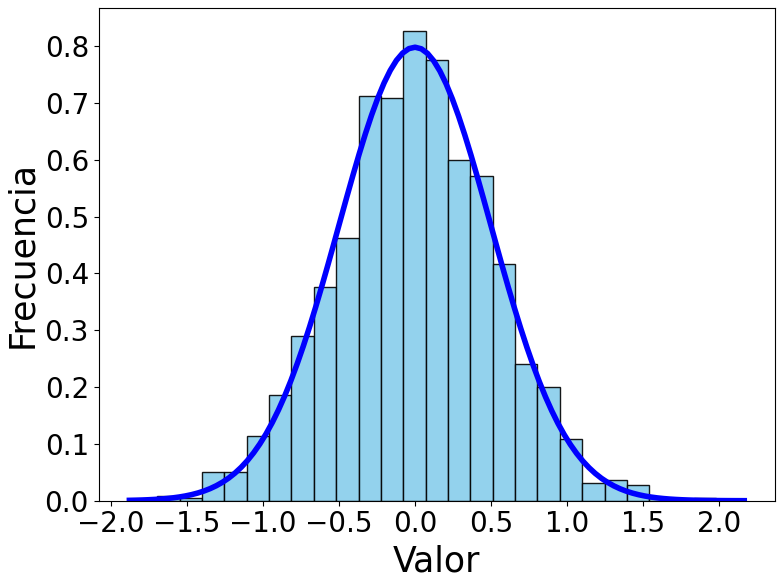
\includegraphics[width=\textwidth]{img/experiments/unimodal.png}
        \caption{Distribución unimodal.}\label{fig:unimodal}
    \end{subfigure}
    \hfill
    \begin{subfigure}[b]{0.43\textwidth}
        \centering
        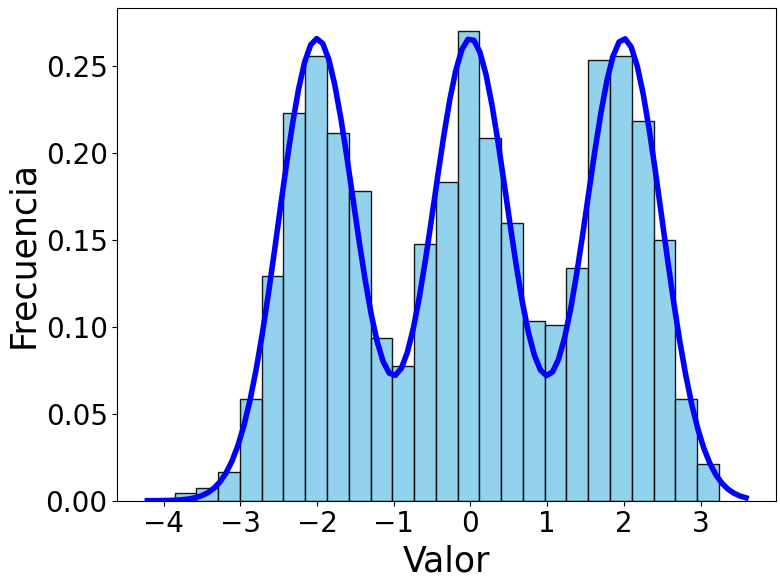
\includegraphics[width=\textwidth]{img/experiments/multimodal.png}
        \caption{Distribución multimodal con tres modas.}\label{fig:multimodal}
    \end{subfigure}
    \caption[Comparación de distribuciones unimodal y multimodal.]{Ejemplos de distribuciones unimodal y multimodal. La distribución unimodal muestra un único máximo, mientras que la distribución multimodal presenta tres máximos, cada uno correspondiente a una moda.}\label{fig:unimodal-multimodal}
\end{figure}

\subsection{Distribución Normal}
La distribución normal, o distribución de Gauss, es la distribución de probabilidad más estudiada y utilizada en el ámbito de la inferencia estadística~\cite{Bryc1995TheND}, dadas sus propiedades matemáticas, como su simetría, la concentración de probabilidades alrededor de la media y su relación con otras distribuciones.

\begin{definicion}[Distribución normal]
    Sea $X$ una variable aleatoria continua. Decimos que $X$ sigue una \emph{distribución normal} si su función de densidad $f_X$ viene dada por:

    \[ f_X(x) = \frac{1}{\sqrt{2\pi \sigma^2}} \cdot e^{-\frac{{(x - \mu)}^2}{2\sigma^2}}, \]

    donde $\mu, \sigma^2 \in \mathbb{R}$ denotan, respectivamente, la esperanza y varianza de la variable aleatoria $X$.

    Además, si $X$ sigue una distribución normal, lo denotaremos como $X \sim \mathcal{N}(\mu,\sigma^2)$. De igual modo, si $\mu = 0$ y $\sigma^2=1$, entonces diremos que la variable aleatoria $X \sim \mathcal{N}(0,1)$ sigue una \emph{distribución normal estándar}.
\end{definicion}

\begin{proposicion}
    Si $X \sim \mathcal{N}(\mu,\sigma^2)$, entonces la variable aleatoria $X$ satisface las siguientes propiedades:

    \begin{itemize}
        \item La distribución es simétrica respecto de su media $\mu$.
        \item La moda coincide con la media.
        \item $P[\mu - \sigma < X < \mu + \sigma] \approx 0,6826$.
        \item $P[\mu - 2\sigma < X < \mu + 2\sigma] \approx 0,9544$.
        \item $P[\mu - 3\sigma < X < \mu + 3\sigma] \approx 0,9974$.
        \item Si $a, b \in \mathbb{R}$, entonces $aX + b \sim \mathcal{N}(a\mu + b, a^2\sigma^2)$.
    \end{itemize}
\end{proposicion}

Como consecuencia de la primera propiedad de la proposición anterior, se pueden relacionar todas las variables aleatorias normales con la distribución $\mathcal{N}(0,1)$.

\begin{proposicion}
    Sea $X \sim \mathcal{N}(\mu,\sigma^2)$. Entonces,
    
    \[ Z = \frac{X-\mu}{\sigma} \]

    es una variable aleatoria que sigue una distribución normal estándar $Z \sim\mathcal{N}(0,1)$.
\end{proposicion}

\begin{figure}[h]
    \centering
    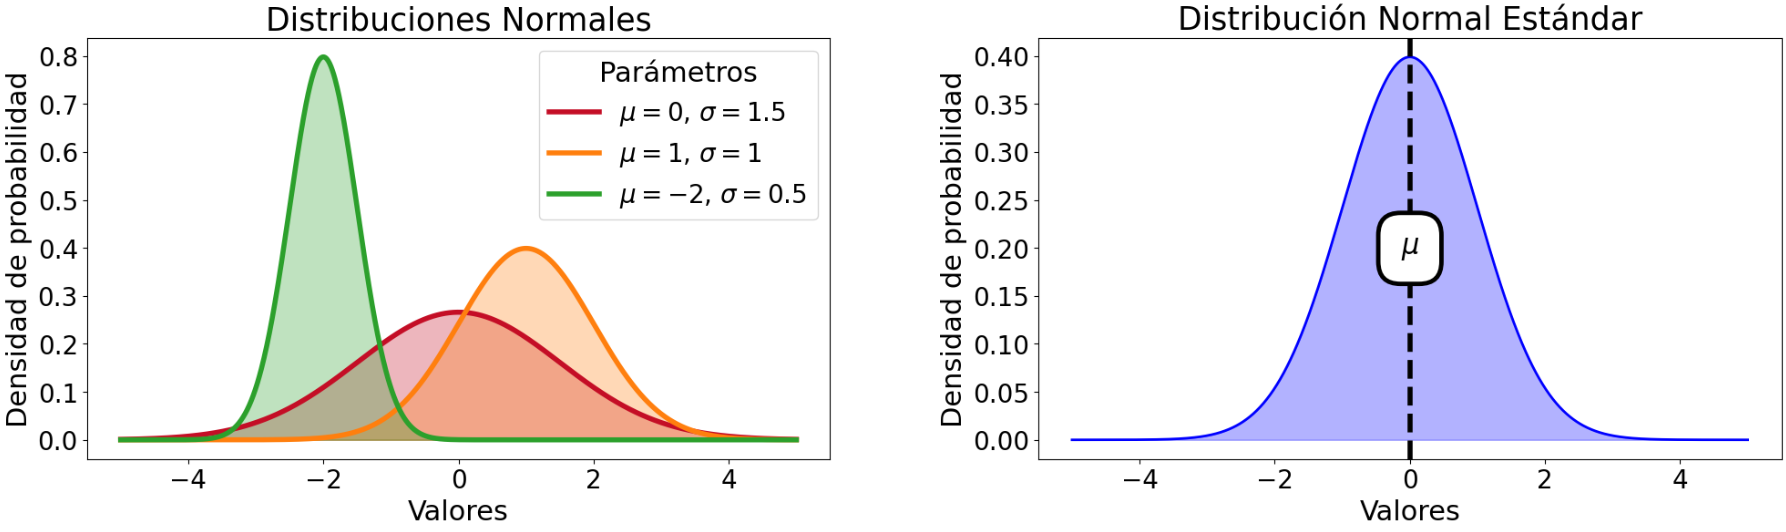
\includegraphics[width=0.9\textwidth]{img/distribuciones-normales.png}
    \caption[Ejemplos de distribuciones normales.] {Ejemplos de distribuciones normales. A la izquierda, observamos distintas distribuciones normales, donde podemos notar como el parámetro $\mu$ determina el centro de la distribución y el parámetro $\sigma$ controla la dispersión de los datos. A medida que el parámetro $\sigma$ incrementa, la distribución se vuelve más dispersa y su altura máxima disminuye. A la derecha, observamos una distribución normal estándar, donde se puede apreciar con claridad que la distribución es simétrica con respecto a $\mu$.}\label{fig:distribuciones-normales}
\end{figure}

\subsection{Distribución de Rademacher}\label{subsec:distribucion-rademacher}
La distribución de Rademacher es una distribución de probabilidad discreta que se utiliza ampliamente en la teoría del aprendizaje estadístico, particularmente en el análisis de la capacidad de generalización de los modelos.

\begin{definicion}[Distribución de Rademacher]
    Sea $X$ una variable aleatoria discreta. Decimos que $X$ sigue una \emph{distribución de Rademacher} si toma los valores $+1$ y $-1$ con igual probabilidad, es decir,

    \[
        P[X = 1] = P[X = -1] = \frac{1}{2}.
    \]

    En tal caso, denotamos esta variable como $X \sim \text{Rad}$.
\end{definicion}

\begin{proposicion}
    Si $X \sim \text{Rad}$, entonces $X$ es una variable aleatoria simétrica respecto al origen, con esperanza $\mathbb{E}[X] = 0$ y varianza $\text{Var}(X) = 1$.
\end{proposicion}

\begin{proposicion}
    Sean $X_1, \dots, X_n$ variables independientes con $X_i \sim \text{Rad}$. Entonces, para cualquier conjunto de constantes $a_1, \dots, a_n \in \mathbb{R}$, la variable

    \[
        S = \sum_{i=1}^n a_i X_i
    \]

    es una combinación lineal de variables de Rademacher con esperanza cero y varianza $\sum_{i=1}^n a_i^2$.
\end{proposicion}


\chapter{Descomposición en Valores Singulares y Pseudoinversa de una Matriz}\label{ch:descomposicion-valores-singulares-pseudoinversa}

En este capítulo presentaremos dos conceptos fundamentales de cara al desarrollo del trabajo: la descomposición en valores singulares (SVD) y la pseudoinversa de una matriz. En cuanto a las referencias utilizadas a lo largo de este capítulo, debemos destacar~\cite{Friedberg2014linear, Strang2023, Poole2011}. Estos libros nos han ayudado a presentar los conceptos básicos más importantes, así como las demostraciones de los resultados más relevantes del capítulo.

\section{Vectores y matrices}\label{sec:vectores-matrices}

En primer lugar, repasaremos la notación que utilizaremos para vectores y matrices, así como los principales tipos de matrices con las que trabajaremos. Además, recordaremos las condiciones bajo las cuales una matriz posee inversa.

Trabajaremos siempre con escalares reales y escribiremos los vectores de $\mathbb{R}^{n}$ como vectores columna en lugar de vectores fila. Es decir, si $v \in \mathbb{R}^{n}$, entonces

\[ 
    v = \begin{pmatrix} 
        v_{1} \\ 
        v_{2} \\ 
        \vdots \\
        v_{n}
    \end{pmatrix} = {(v_{1}, v_{2}, \ldots, v_{n})}^{T}, \quad \text{donde } v_i \in \mathbb{R} \ \ \forall i \in \{1, \ldots, n \}.
\]

También se recuerdan los conceptos de norma y ortonormalidad de vectores, que serán de gran utilidad en el desarrollo de resultados posteriores. De esta manera, dados dos vectores $u, v \in \mathbb{R}^{n}$, denotaremos por $u \cdot v$ su producto escalar usual y por $\| u \|$ la norma euclídea del vector $u$. Así, diremos que dos vectores son ortogonales si su producto escalar es igual a cero.

Denotaremos por $\mathcal{M}_{m \times n}(\mathbb{R})$ al espacio vectorial de las matrices de orden $m$ por $n$ con entradas en $\mathbb{R}$. A la matriz cuyas entradas son todas iguales a cero la llamaremos matriz cero y la denotaremos por $O$. Además, podemos formar una matriz a partir de vectores columna, utilizando la notación $V = [v_1, v_2, \ldots, v_n]$, donde $\{v_1, v_2, \ldots, v_n\}$ son los vectores columna que componen la matriz V.

\begin{definicion}
    La matriz \textbf{traspuesta} $A^{T}$ de una matriz $A \in \mathcal{M}_{m \times n}(\mathcal{R})$ es la matriz de tamaño $n \times m$ que se obtiene de la matriz $A$ al intercambiar las filas por las columnas, es decir, $(a^{T})_{ij} = a_{ji}$. Decimos que una matriz cuadrada $A$ es \textbf{simétrica} si cumple $A^{T} = A$ y, decimos que es \textbf{ortogonal} si sus columnas están formadas por vectores ortonormales dos a dos.
\end{definicion}

Denotamos la \textbf{delta de Kronecker} $\delta_{ij}$ como la función dada por

\[
    \delta_{ij} =
    \begin{cases}
        1 & \text{si } i = j \leq r, \\
        0 & \text{si } i \neq j.
    \end{cases}
\]

De esta manera, la \textbf{matriz identidad} de tamaño $n \times n$ ($I_{n}$) viene dada por $(I_n)_{ij} = \delta_{ij}$.

\begin{definicion}
    Sea $A$ una matriz de tamaño $m \times n$. Se dice que $A$ es una matriz \textbf{escalonada} si es la matriz $O$, o bien satisface las tres condiciones siguientes:

    \begin{enumerate}
        \item El primer elemento no nulo de cada fila, si existe, es un $1$.
        \item El primer $1$ de la segunda y sucesivas filas está a la derecha del primer $1$ de la fila anterior.
        \item Si tiene filas nulas (compuestas únicamente por ceros), estas aparecen en la parte inferior de la matriz, justo debajo de las filas no nulas.
    \end{enumerate}

    Además, las operaciones elementales que se pueden realizar a una matriz para obtener su forma escalonada son las siguientes:

    \begin{itemize}
        \item Intercambiar dos filas (columnas).
        \item Multiplicar una fila (columna) por un múltiplo distinto de cero.
        \item Sumar un múltiplo de una fila (columna) a otra fila (columna).
    \end{itemize}
\end{definicion}

\begin{definicion}
    Sean $A$ y $B$ dos matrices de tamaño $m \times n$. Se dice que la matriz $A$ es \textbf{equivalente} por filas a la matriz $B$ (o simplemente equivalente) si $B$ se obtiene de $A$ por medio de la aplicación sucesiva de operaciones elementales.
\end{definicion}

\begin{definicion}
    Una matriz $A$ de tamaño $m \times n$ es \textbf{escalonada reducida} si es escalonada y, además, todo elemento en una columna que esté encima del primer uno de cualquier fila es cero.
\end{definicion}

\begin{ejemplo}
    Para matrices cuadradas de tamaño $2$, las posibles matrices escalonadas reducidas son las siguientes:

    \[
        \begin{pmatrix} 0 & 0 \\ 0 & 0 \end{pmatrix}, \quad
        \begin{pmatrix} 1 & 0 \\ 0 & 1 \end{pmatrix}, \quad
        \begin{pmatrix} 1 & $x$ \\ 0 & 0 \end{pmatrix} \quad y \quad
        \begin{pmatrix} 0 & 1 \\ 0 & 0
        \end{pmatrix},
    \]

    donde $x \in \mathbb{R}$ puede ser cualquier escalar.
\end{ejemplo}

Una vez introducidas las definiciones anteriores, disponemos de todas las herramientas necesarias para introducir el concepto de rango de una matriz.

\begin{definicion}[Rango de una matriz]
    Sea $A$ una matriz de tamaño $m \times n$. Se denomina \textbf{rango} de $A$ ($rang(A)$) al número de filas no nulas de la matriz en la forma escalonada reducida equivalente a $A$. De manera equivalente, el rango de una matriz se puede definir como la dimensión del espacio generado por sus vectores fila o columna. De esta manera, el rango de una matriz será igual al número máximo de vectores fila o columna que sean linealmente independientes entre sí.
\end{definicion}

El siguiente resultado nos recuerda cómo utilizar el rango para determinar si una matriz es invertible.

\begin{proposicion}
    Sea $A$ una matriz cuadrada de tamaño $n$, entonces equivalen:

    \begin{enumerate}
        \item $A$ es invertible.
        \item $A$ es equivalente a $I_n$.
        \item El rango de $A$ es $n$.
        \item $\det(A) \neq 0$. Además, si $A$ es invertible, entonces $\det(A^{-1})=\frac{1}{\det(A)}$.
    \end{enumerate}
\end{proposicion}

Finalmente, recordamos algunas de las propiedades de las matrices invertibles.

\begin{proposicion}
    Sean $A$ y $B$ matrices cuadradas e invertibles del mismo tamaño. Entonces se cumple:

    \begin{enumerate}
        \item $A^{-1}$ es invertible y ${(A^{-1})}^{-1} = A$ (la inversa de $A^{-1}$ es la propia matriz $A$).
        \item $A^{T}$ es invertible y ${(A^{T})}^{-1} = {(A^{-1})}^{T}$.
        \item La matriz $AB$ es invertible y ${(AB)}^{-1} = B^{-1}A^{-1}$.
    \end{enumerate}
\end{proposicion}

\begin{definicion}
    Sea $A$ una matriz cuadrada de tamaño $n$. Un vector no nulo $v \in \mathbb{R}^{n}$ se dice que es un \textbf{vector propio} (o autovector) de la matriz $A$ si $Av=\lambda v$ para algún escalar $\lambda \in \mathbb{R}$. Además, el escalar $\lambda$ se llama \textbf{valor propio} (o autovalor) de la matriz $A$ correspondiente al vector propio $v$. Recordemos que $\lambda$ es un valor propio de $A$ si, y solo si, $det(A-\lambda I_n)=0$.
\end{definicion}

Para cualquier matriz $A \in \mathcal{M}_{m \times n}(\mathbb{R})$, la matriz $A^{T}A$ es simétrica y, en consecuencia, es diagonalizable ortogonalmente (teorema espectral real~\cite{Blum2021}). Se comprueba de manera sencilla que todos los valores propios de la matriz $A^{T}A$ son no negativos.

\section{SVD y pseudoinversa}\label{sec:svd-pseudoinversa}

LLegados a este punto, ya podemos presentar los principales contenidos sobre matrices abordados en este trabajo: la descomposición en valores singulares y la pseudoinversa. Cabe destacar que estos resultados se enuncian para matrices con escalares en el cuerpo $\mathbb{R}$, aunque su generalización a otros cuerpos es posible.

\begin{definicion}
    Si $A$ es una matriz de tamaño $m \times n$, los \textbf{valores singulares} de $A$ son las raíces cuadradas (positivas) de los valores propios de la matriz $A^{T}A$, y se denotan mediante $\sigma_{1}, \sigma_{2}, \ldots, \sigma_{n}$. Además, es convencional ordenar los valores singulares de manera que $\sigma_{1} \geq \sigma_{2} \geq \cdots \geq \sigma_{n}$.
\end{definicion}


El siguiente resultado nos indica que toda matriz, independientemente de su estructura, puede ser factorizada como producto de tres matrices, dos de las cuales serán ortogonales.

\begin{teorema}[Descomposición en valores singulares]
    Sea $A \in \mathcal{M}_{m \times n}(\mathbb{R})$ una matriz cuyo rango es $r$ y con valores singulares positivos $\sigma_{1} \geq \sigma_{2} \geq \cdots \geq \sigma_{r}$, y sea $\Sigma$ la matriz de tamaño $m \times n$ definida por 

    \[
        \Sigma_{ij} =
        \begin{cases}
            \sigma_i & \text{si } i = j \leq r, \\
            0 & \text{en otro caso.}
        \end{cases}
    \]

    Entonces existen matrices ortogonales $U$ y $V$ de tamaño $m\times m$ y $n\times n$, respectivamente, de manera que

    \[
        A = U \Sigma V^{T}.
    \]

    A esta factorización la llamaremos \textbf{descomposición en valores singulares (SVD)} de $A$.
\end{teorema}

\begin{proof}
    La demostración se fundamenta en la construcción directa de las matrices $V$ y $U$, verificando posteriormente que se satisface el resultado buscado.

    Para construir la matriz ortogonal $V$, basta tomar una base ortonormal $\{v_1, v_2, \ldots, v_n \}$ de $\mathbb{R}^{n}$ formada por vectores asociados a los valores propios $\{\lambda_1, \lambda_2, \ldots, \lambda_n\}$ de la matriz simétrica y cuadrada $A^{T}A$ de tamaño $n$. Entonces, se tiene que $V = [v_1, v_2, \ldots, v_n]$ es una matriz ortogonal y cuadrada de tamaño $n$.

    Para construir la matriz ortogonal $U$, primero notemos que $\{Av_1, Av_2, \ldots, Av_n \}$ es un conjunto ortogonal de vectores de $\mathbb{R}^{m}$. En efecto, para $i \neq j$, se cumple

    \[ (Av_i)\cdot(Av_j) = (Av_i)^{T}Av_j=v_{i}^{T}A^{T}Av_j = v_{i}^{T}\lambda_j v_j=\lambda_j(v_i \cdot v_j) = 0,\]

    dado que los vectores propios $v_i$ son ortogonales. Recordamos ahora que los valores singulares satisfacen $\sigma_i = ||Av_i||$ y que los primeros $r$ valores singulares son distintos de cero. Por tanto, podemos normalizar $Av_1, \ldots, Av_r$ de la siguiente forma:

    \begin{equation}
        u_i = \frac{1}{\sigma_i} A v_i, \quad \text{para } i = \{1, \ldots, r\}.
        \label{eq:singulares1}
    \end{equation}
    

    Esto garantiza que $\{ u_1, \ldots, u_r\}$ es un conjunto ortonormal de $\mathbb{R}^{m}$, pero si $r < m$ no será una base para $\mathbb{R}^{m}$. En este caso, se extiende el conjunto $\{u_1, \ldots, u_r \}$ a una base ortonormal $\{u_1, \ldots, u_m \}$ para $\mathbb{R}^{m}$. En consecuencia, la matriz $U$ es ortogonal. Ahora, falta comprobar que, con la construcción realizada, se satisface el resultado $A = U \Sigma V^{T}$. Dado que $V^{T} = V^{-1}$ (al ser la matriz $V$ ortogonal), esto equivale a demostrar que $AV = U\Sigma$.

    En primer lugar, sabemos, a partir de la ecuación~\eqref{eq:singulares1}, que $Av_i=\sigma_i u_i$ para $i=\{1, \ldots, r\}$ y que $||A v_i|| = \sigma_i = 0$ para $i=\{r+1, \ldots,n\}$. En consecuencia, $Av_i = 0$ para $i=\{r+1, \ldots,n\}$. Por tanto,

    \begin{align*}
        A V &= A \begin{bmatrix} \mathbf{v}_1 & \cdots & \mathbf{v}_n \end{bmatrix} \\
            &= \begin{bmatrix} A \mathbf{v}_1 & \cdots & A \mathbf{v}_n \end{bmatrix} \\
            &= \begin{bmatrix} A \mathbf{v}_1 & \cdots & A \mathbf{v}_r & 0 & \cdots & 0 \end{bmatrix} \\
            &= \begin{bmatrix} \sigma_1 \mathbf{u}_1 & \cdots & \sigma_r \mathbf{u}_r & 0 & \cdots & 0 \end{bmatrix} \\
            &= \begin{bmatrix} \mathbf{u}_1 & \cdots & \mathbf{u}_m \end{bmatrix}
               \begin{bmatrix} 
                   \sigma_1 & \cdots & 0 & O \\
                   \vdots & \ddots & \vdots & O \\
                   0 & \cdots & \sigma_r & O \\
                   O & O & O & O
               \end{bmatrix} \\
            &= U \Sigma,
    \end{align*}

    quedando probada la igualdad $AV = U \Sigma$.
\end{proof}

El siguiente resultado generaliza el concepto de matriz inversa cuando la matriz no es cuadrada.
\begin{definicion}[Pseudoinversa]
    Sea $A \in \mathcal{M}_{m \times n}(\mathbb{R})$ con $m > n$ y cuyas columnas son linealmente independientes. Se define la \textbf{pseudoinversa} (o inversa de Moore-Penrose) de la matriz $A$ como la matriz $A^{\dagger}$ dada por

    \[ A^{\dagger} = {(A^{T}A)}^{-1}A^{T}, \]

    donde se puede comprobar que $A^{\dagger} \in \mathcal{M}_{n \times m}(\mathbb{R})$.
\end{definicion}

No obstante, dado que toda matriz se puede factorizar en su descomposición en valores singulares, podemos definir la pseudoinversa de una matriz a partir de dicha factorización.
\begin{definicion}
    Sea $A$ una matriz de tamaño $m \times n$ de rango $r$ con descomposición en valores singulares $A = U \Sigma V^{T}$ y con valores singulares distintos de cero $\sigma_{1} \geq \sigma_{2} \geq \cdots \geq \sigma_{r}$. Sea $\Sigma^{\dagger}$ la matriz de tamaño $n \times m$ definida por

    \[
        \Sigma^{\dagger}_{ij} =
        \begin{cases}
            \frac{1}{\sigma_i} & \text{si } i = j \leq r, \\
            0 & \text{en otro caso.}
        \end{cases}
    \]

    Entonces la factorización $A^{\dagger} = V \Sigma^{\dagger} U^{T}$ es una descomposición en valores singulares de $A^{\dagger}$, donde $\Sigma^{\dagger}$ es la pseudoinversa de $\Sigma$. Además, $A^{\dagger}$ es la pseudoinversa de $A$.
\end{definicion}

Presentamos una forma análoga de definir la pseudoinversa de una matriz, basándose en las propiedades que debe cumplir la pseudoinversa, que serán de gran utilidad en el desarrollo del trabajo.
\begin{definicion}[Condiciones de Moore-Penrose]
    Sea $A \in \mathcal{M}_{m \times n}(\mathbb{R})$ la pseudoinversa de $A$, $A^{\dagger} \in \mathcal{M}_{n \times m}(\mathbb{R})$, es la única matriz que satisface las siguientes propiedades, conocidas como las \textbf{condiciones de Moore-Penrose}:

    \begin{enumerate}
        \item $A A^{\dagger} A = A$.
        \item $A^{\dagger} A A^{\dagger} = A^{\dagger}$.
        \item ${(A A^{\dagger})}^{T}$ y ${(A^{\dagger} A)}^{T}$ son simétricas.
    \end{enumerate}

    En particular, se tiene que $AA^{\dagger}$ y $A^{\dagger}A$ son proyecciones ortogonales sobre $Im(A)$ y ${Im(A)}^{T}$ respectivamente. Además, si $A$ es de rango completo, es decir, $rango(A) = r  = \min\{m, n\}$, entonces $A^{\dagger}$ puede expresarse de forma sencilla como sigue:

    \begin{itemize}
        \item Si $r = m = n$, entonces la matriz $A$ es invertible y $A^{\dagger} = A^{-1}$.
        \item Si $r = m < n$, entonces $A$ tiene filas linealmente independientes (la aplicación lineal asociada a $A$ es sobreyectiva y $AA^{T}$ es invertible) y $A^{\dagger} = A^{T}{(AA^{T})}^{-1}$.
        \item Si $r = n < m$, entonces $A$ tiene columnas linealmente independientes (la aplicación lineal asociada a $A$ es inyectiva y $A^{T}A$ es invertible) y $A^{\dagger} = {(A^{T}A)}^{-1} A^{T}$.
    \end{itemize}
\end{definicion}

A continuación, se presentan dos propiedades de la pseudoinversa que son fundamentales para comprender la estructura de la solución de sistemas lineales.

\begin{lema}\label{lema:propiedades-pseudoinversa}
    Para una matriz $A \in \mathcal{M}_{m \times n}(\mathbb{R})$, se verifica:

    \begin{enumerate}
        \item $\operatorname{Im}(I-A^{\dagger}A) = \ker(A)$.
        \item $\ker(A^{\dagger}) = \ker(A^{T})$.
    \end{enumerate}

    Donde $\operatorname{Im(A)}$ y $\ker(A)$ denotan, respectivamente, la imagen y el núcleo de la aplicación lineal asociada a la matriz $A$.
\end{lema}

Finalmente, la solución de norma mínima para un problema de mínimos cuadrados puede definirse mediante la pseudoinversa de una matriz, como se establece en el siguiente teorema. Más adelante, este resultado será de gran utilidad para obtener la mejor aproximación en problemas de regresión.

\begin{teorema}
    El problema de mínimos cuadrados $A\mathbf{x}=\mathbf{b}$, con $A \in \mathcal{M}_{m \times n}(\mathbb{R})$, $\mathbf{x} \in \mathbb{R}^{n}$ y $\mathbf{b} \in \mathbb{R}^{m}$, tiene una solución única $\bar{x}$ de mínimos cuadrados con norma mínima dada por

    \[ \bar{\mathbf{x}} = A^{\dagger}\mathbf{b}. \]
\end{teorema}

\begin{proof}
    Sea $A \in \mathcal{M}_{m \times n}(\mathbb{R})$ con $rang(A) = r$ y sea $U\Sigma V^{T}$ su descomposición en valores singulares. De este modo, se tiene que $A^{\dagger} = V \Sigma^{\dagger} U^{T}$. Sean $\mathbf{y}=V^{T}\mathbf{x}$ y $\mathbf{c}=U^{T}\mathbf{b}$, expresados de la siguiente forma

    \[
        \mathbf{y} = \begin{bmatrix} \mathbf{y}_1 \\ \mathbf{y}_2 \end{bmatrix}, \quad 
        \mathbf{c} = \begin{bmatrix} \mathbf{c}_1 \\ \mathbf{c}_2 \end{bmatrix},
    \]

    donde $\mathbf{y_1}, \mathbf{c_1} \in \mathbb{R}^{r}$.

    Se busca minimizar $\|\mathbf{b} - A \mathbf{x}\|$ o, de manera equivalente, $\|\mathbf{b} - A \mathbf{x}\|^2$. Usando que $U^T$ es ortogonal (dado que $U$ es ortogonal), se tiene  

    \[
        \|\mathbf{b} - A \mathbf{x}\|^2 = \| U^T (\mathbf{b} - A \mathbf{x}) \|^2 = \| U^T (\mathbf{b} - U \Sigma V^T \mathbf{x}) \|^2 = \| U^T \mathbf{b} - U^T U \Sigma V^T \mathbf{x} \|^2
    \]

    \[
        = \|\mathbf{c} - \Sigma \mathbf{y}\|^2 = \left\| \begin{bmatrix} \mathbf{c}_1 \\ \mathbf{c}_2 \end{bmatrix} - \begin{bmatrix} D & O \\ O & O \end{bmatrix} \begin{bmatrix} \mathbf{y}_1 \\ \mathbf{y}_2 \end{bmatrix} \right\|^2 = \left\| \begin{bmatrix} \mathbf{c}_1 - D \mathbf{y}_1 \\ \mathbf{c}_2 \end{bmatrix} \right\|^2.
    \]

    Dado que sólo disponemos de control sobre $\mathbf{y}_1$, el valor mínimo ocurre cuando $\mathbf{c}_1 - D \mathbf{y}_1 = 0$ o, de manera equivalente, cuando $\mathbf{y}_1 = D^{-1} \mathbf{c}_1$. De modo que todas las soluciones $\mathbf{x}$ de mínimos cuadrados son de la forma  

    \[
        \mathbf{x} = V \mathbf{y} = V \begin{bmatrix} D^{-1} \mathbf{c}_1 \\ \mathbf{y}_2 \end{bmatrix}.
    \]

    Definimos $\bar{\mathbf{x}} = V \bar{\mathbf{y}} = V \begin{bmatrix} D^{-1} \mathbf{c}_1 \\ 0 \end{bmatrix}$ y afirmamos que $\bar{\mathbf{x}}$ es la solución de mínimos cuadrados de norma mínima. Para demostrarlo, supongamos que $\mathbf{x}^{\prime}=V\mathbf{y}^{\prime} = V \begin{bmatrix} D^{-1} \mathbf{c}_1 \\ y_2 \end{bmatrix}$ es otra solución diferente al problema de mínimos cuadrados (por tanto, $\mathbf{y}_2 \neq 0$). Entonces, se verifica

    \[ \| \bar{\mathbf{x}} \| = \| V\bar{\mathbf{y}} \| = \| \bar{\mathbf{y}} \| < \| {\mathbf{y}^{\prime}} \| = \| V\mathbf{y}^{\prime} \| = \| \mathbf{x}^{\prime} \|,\]

    como se quería probar. Por último, falta demostrar que $\bar{\mathbf{x}}$ es igual a $A^{\dagger}\mathbf{b}$. Para ello, basta calcular

    \[ \bar{\mathbf{x}} = V\bar{\mathbf{y}} = V \begin{bmatrix} D^{-1} \mathbf{c}_1 \\ 0 \end{bmatrix} = V \begin{bmatrix} D^{-1} & O \\ O & O \end{bmatrix} \begin{bmatrix} \mathbf{c}_1 \\ \mathbf{c}_2 \end{bmatrix} = V \Sigma^{\dagger} \mathbf{c} = V \Sigma^{\dagger} U^{T} \mathbf{b} = A^{\dagger}\mathbf{b}.\]

    
\end{proof}

% \chapter{Aproximación lineal}\label{ch:capitulo-aproximacion-lineal}

\endinput